\begin{figure}[h]
    \centering
    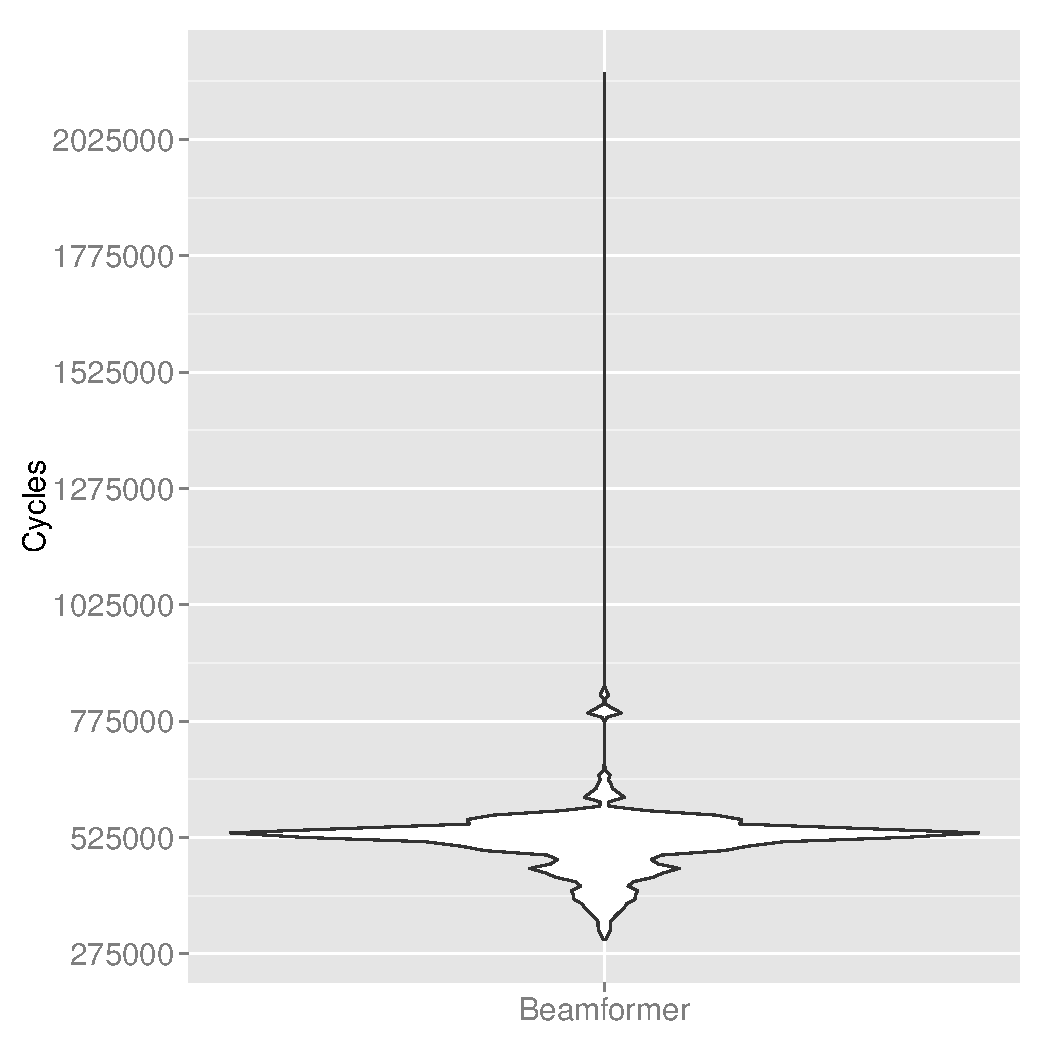
\includegraphics[width=0.7\textwidth]{streamit-paper/graphics/beamformer_motivation.pdf}
    \caption{Distribution of the runtime for Beamformer resulting from an exhaustively exploration of the hardware/software co-design space.
     The application has been partitioned into different number of threads and core compositions.}
     \label{fig:beamformermotiv}
\end{figure}

\begin{figure}[h]
    \centering
    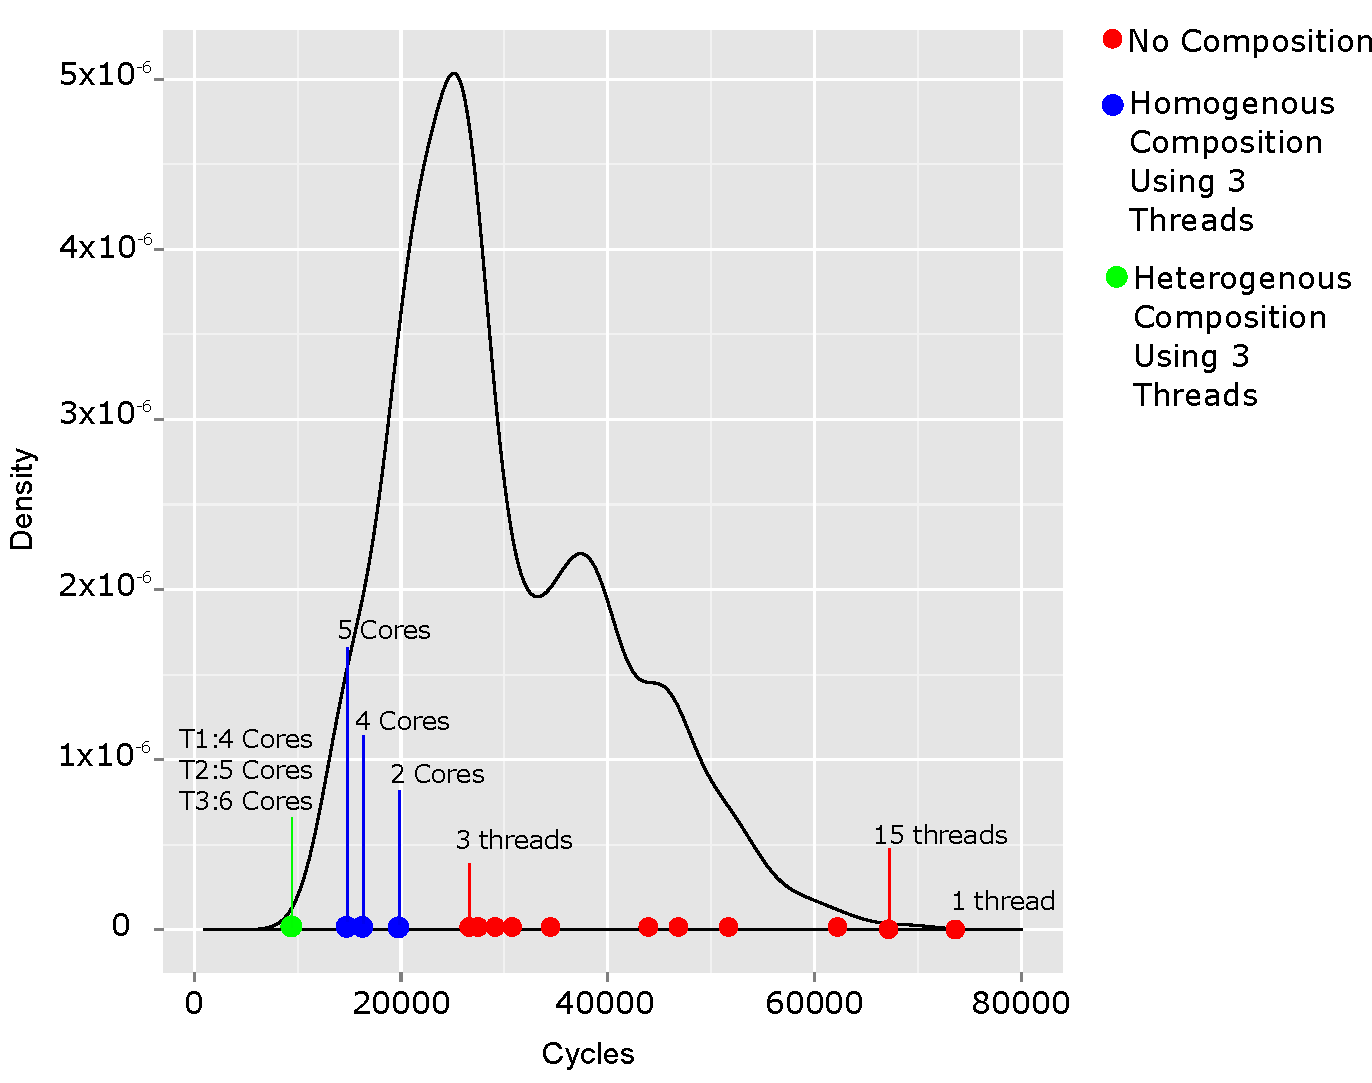
\includegraphics[width=1\textwidth]{streamit-paper/graphics/temp_motivation_3.pdf}
    \caption{Distribution of the runtime for FilterBank with different core composition and thread pairings. The dots on the X-axis represent specific configurations and their cycle counts.}
     \label{fig:threadcoremotiv}
\end{figure}

In this section, the difficulty of finding a good mixture of thread partitioning and core allocation is illulstrated in two examples.
First, a simple experiment is conducted where one StreamIt benchmark is taken, \bench{Beamformer}.
The benchmark's tasks are partitioned into threads and a various number of cores are allocated to each thread.
A co-design of more than 32,000 combinations (exhaustive space) of thread mappings and core compositions pairings is generated.
Each design point is executed on the dynamic multicore simulator, the exact details about the experimental setup are presented later in section~\ref{sec:setup}.

Figure~\ref{fig:beamformermotiv} presents the distribution of the execution times, displayed as cycles, from the co-design space as a violin plot.
An intuitive way to think about this violin plot is to consider it as a smoothed histogram rotated by 90 degrees and mirrored.
The majority of the sampled points have a cycle count of around 525,000 cycles with the worst points taking more than 2 millions cycles.
The best performance is around 275,000 cycles which is 2x faster than the majority of the data points.
It is important to notice how there are only a few sample points that approach the fastest execution times.
This underlines the notion that finding a combination of threads and cores is a non-trivial endeavour, as randomly choosing a configuration will result in a suboptimal performance.
It also demonstrates that an incorrect decision may result in considerable slow-down compared to the average execution time.

%Insert an example to show that it's a mix of threads and cores that matters.
Whilst there exists a large variety thread-core combinations, certain heuristics can be used to try and minimize the space.
For example, choosing only combinations that lead to homogeneous core compositions reduces the search space to only 49 possible solutions.
However, as shown in Figure~\ref{fig:threadcoremotiv} limiting the space will limit performance.
Figure~\ref{fig:threadcoremotiv} shows the performance distribution of different core-thread pairings for the \bench{FilterBank} StreamIt benchmark.
Similar to Figure~\ref{fig:beamformermotiv}, the X-axis represents a certain execution time in cycles, whilst the Y-axis represents how frequently different thread-core combinations lead to such a performance.
In this graph, different points are added to the X-axis to demonstrate specific configurations of the processor.
Their location on the X-axis represents the execution time for that specific configuration.
The points represent a set of different heuristics such as only using multithreading, using homogeneous core-compositions with threads and using heterogeneous core-compositions with threads.
In the the case of using core-composition, the configurations are plotted using 3 threads, which was the optimal number of threads for the benchmark.
As can be seen, using only multithreading can lead to some performance improvements, however it will not result in the optimal performance.
Using homogeneous core-compositions for 3 threads does perform better than only using 3 threads, however it still does not obtain the best performance.
In the end, using a heterogeneous configuration leads to a 1.5x speedup compared to the fastest homomgeneous configuration.
Therefore, it is important to consider all possible configurations to ensure the possibility of obtaining the best performance.\\

These two examples illustrates the necessity for designing the technique to predict both the optimal number of threads and core composition to use.
The next section will present a more in-depth analysis of the design space before presenting our machine-learning predictive model.

